\documentclass[11pt]{article}
\usepackage[margin=1in]{geometry}
\usepackage{graphicx,booktabs,amsmath,float}
\usepackage[table]{xcolor}
\title{Image-Space Residual INR: Follow-up Pixel-Supervision Sweep}
\author{Patient-Specific Residual INR --- slam (change\_extent=0)}
\date{\today}
\begin{document}\maketitle
\section*{Setup}
The current (follow-up) image is reconstructed in image space as $\hat{x} = f_\theta^{\mathrm{prior}} + r_\phi$, with the prior INR $f_\theta^{\mathrm{prior}}$ fit to the registered DICOM prior and frozen. The residual $r_\phi$ is trained using only a fraction $p$ of the follow-up pixels (chosen uniformly at random) and evaluated on the full image. Baselines: \textbf{prior-copy} (DICOM prior, uses $0\%$ of the follow-up) and \textbf{prior-finetune} (NeRP-style: the prior INR itself, initialized on the DICOM, fine-tuned on the same observed follow-up pixels).
\begin{table}[H]\centering
\caption{Reconstruction of the full follow-up image vs.\ supervision fraction $p$ (higher PSNR/SSIM better; lower NMSE/CPE better; PBS $\approx 1$ preserves change, $\ll 1$ suppresses it).}
\begin{tabular}{llrrrrrr}
\toprule
$p$ (pixels) & method & PSNR & SSIM & NMSE & CPE & PBS \\
\midrule
25\% & prior-copy & 24.22 & 0.826 & 0.0707 & 0.0268 & 0.000 \\
 & prior-finetune (NeRP) & 29.03 & 0.888 & 0.0234 & 0.0156 & 1.093 \\
 & \textbf{prior+residual (ours)} & 29.33 & 0.860 & 0.0218 & 0.0162 & 0.887 \\
\midrule
50\% & prior-copy & 24.22 & 0.826 & 0.0707 & 0.0268 & 0.000 \\
 & prior-finetune (NeRP) & 32.08 & 0.930 & 0.0116 & 0.0100 & 1.046 \\
 & \textbf{prior+residual (ours)} & 31.34 & 0.897 & 0.0137 & 0.0124 & 0.941 \\
\midrule
75\% & prior-copy & 24.22 & 0.826 & 0.0707 & 0.0268 & 0.000 \\
 & prior-finetune (NeRP) & 35.55 & 0.961 & 0.0052 & 0.0059 & 1.020 \\
 & \textbf{prior+residual (ours)} & 34.20 & 0.908 & 0.0071 & 0.0094 & 0.979 \\
\midrule
100\% & prior-copy & 24.22 & 0.826 & 0.0707 & 0.0268 & 0.000 \\
 & prior-finetune (NeRP) & 49.02 & 0.989 & 0.0002 & 0.0022 & 1.003 \\
 & \textbf{prior+residual (ours)} & 36.68 & 0.919 & 0.0040 & 0.0077 & 0.988 \\
\bottomrule
\end{tabular}\end{table}
\begin{table}[H]\centering
\caption{How well the learned residual recovers the true interval change $(|x_{\mathrm{ref}}|-|x_{\mathrm{prior}}|)$ for the ours model.}
\begin{tabular}{lrr}\toprule
$p$ (pixels) & corr & rel-L1 \\ \midrule
25\% & 0.818 & 0.638 \\
50\% & 0.890 & 0.493 \\
75\% & 0.943 & 0.385 \\
100\% & 0.967 & 0.321 \\
\bottomrule\end{tabular}\end{table}
\section*{Prior INR reconstruction}
\begin{figure}[H]\centering
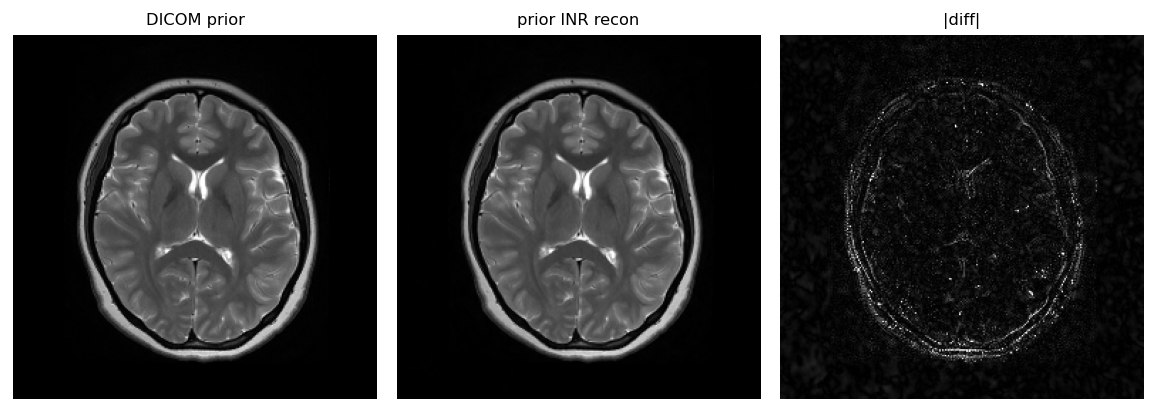
\includegraphics[width=\linewidth]{prior_recon.png}
\caption{The frozen prior INR and the DICOM image it reconstructs.}
\end{figure}
\section*{Qualitative results (ours) per supervision fraction}
\begin{figure}[H]\centering
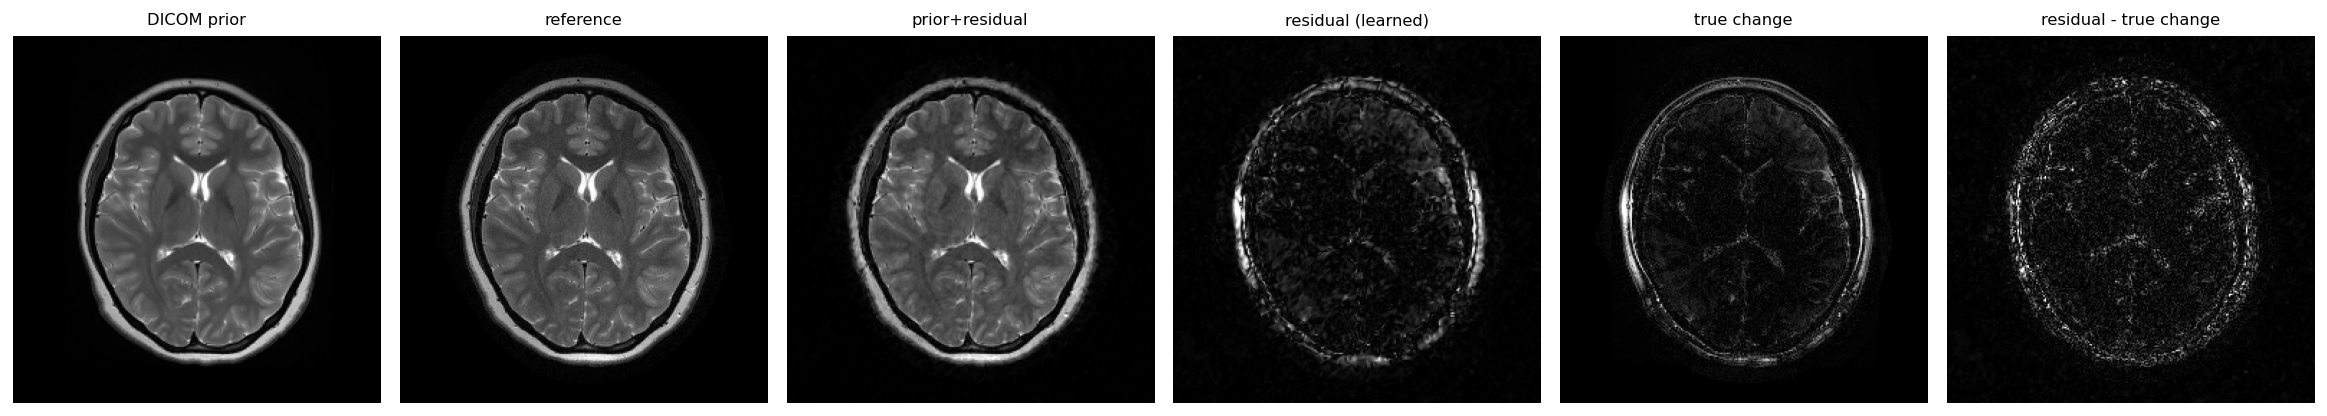
\includegraphics[width=\linewidth]{panel_p025.png}
\caption{$p=25\%$ of follow-up pixels observed. Left to right: DICOM prior, reference follow-up, our reconstruction ($f^{\mathrm{prior}}+r$), learned residual $r$, true change, and the error $|r-\text{true change}|$.}
\end{figure}
\begin{figure}[H]\centering
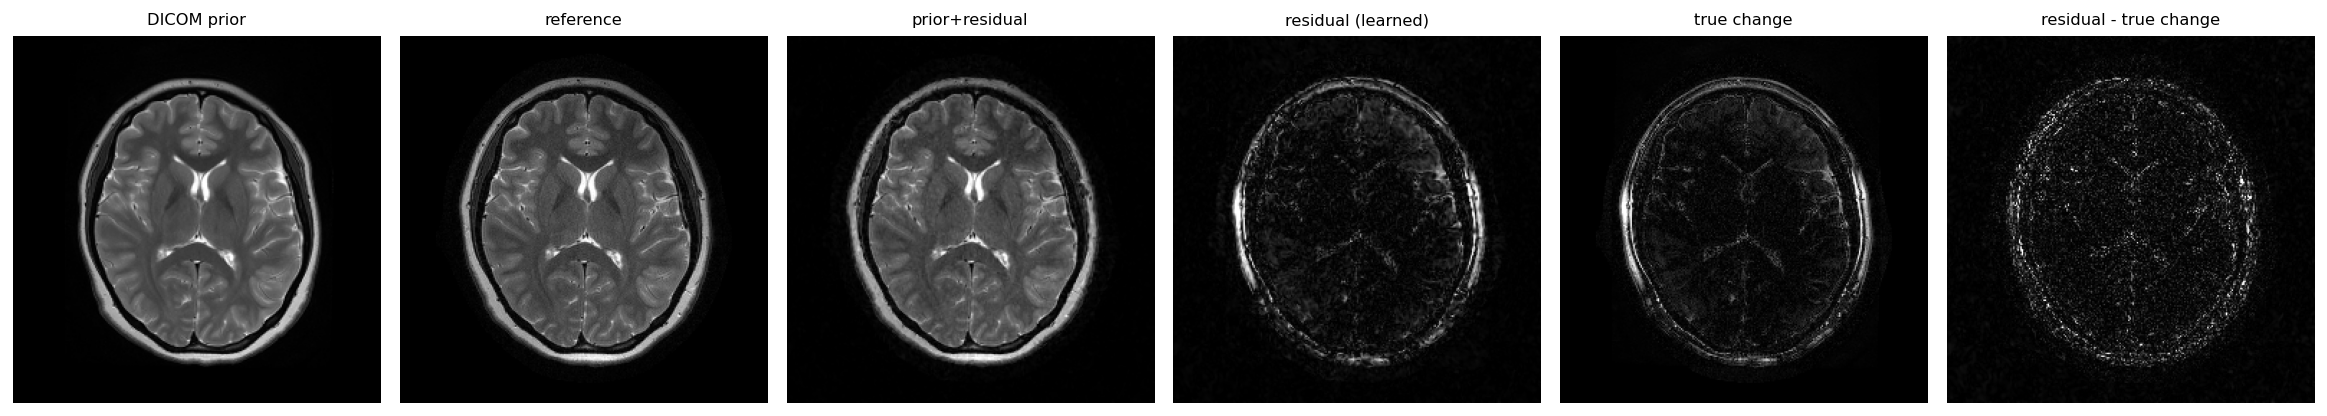
\includegraphics[width=\linewidth]{panel_p050.png}
\caption{$p=50\%$ of follow-up pixels observed. Left to right: DICOM prior, reference follow-up, our reconstruction ($f^{\mathrm{prior}}+r$), learned residual $r$, true change, and the error $|r-\text{true change}|$.}
\end{figure}
\begin{figure}[H]\centering
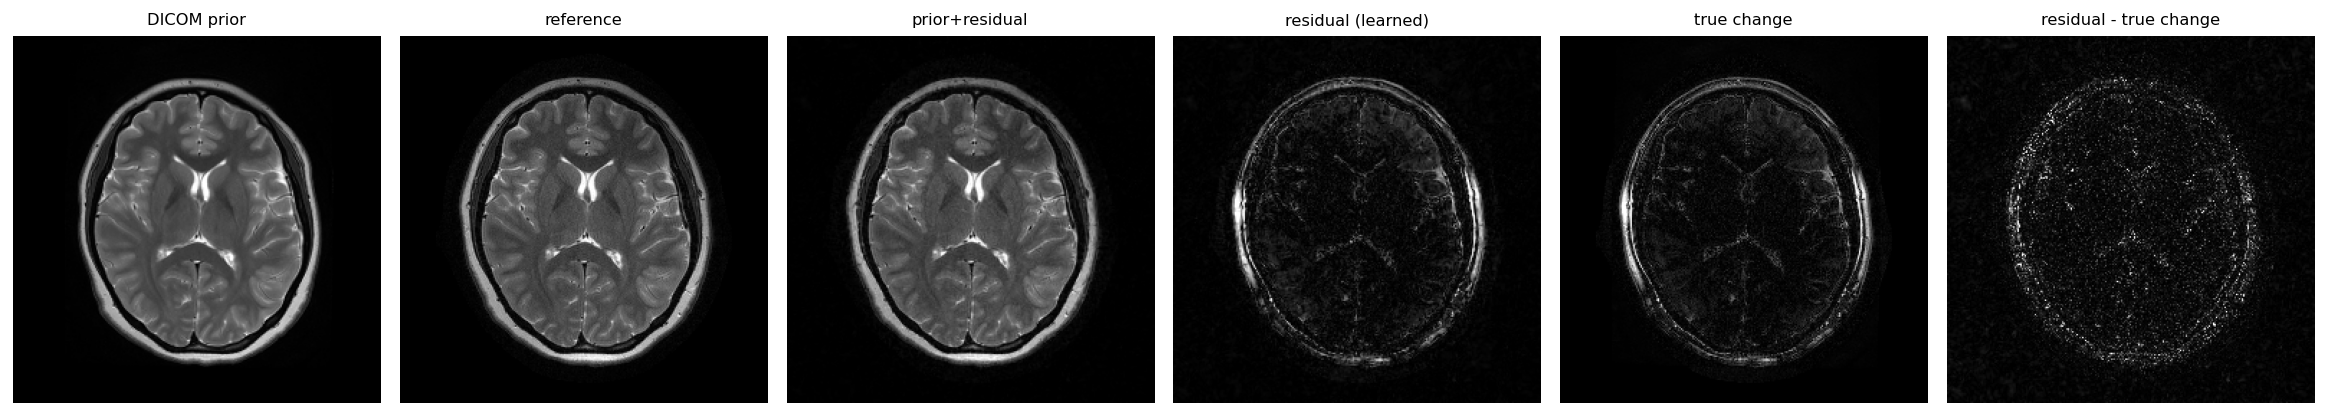
\includegraphics[width=\linewidth]{panel_p075.png}
\caption{$p=75\%$ of follow-up pixels observed. Left to right: DICOM prior, reference follow-up, our reconstruction ($f^{\mathrm{prior}}+r$), learned residual $r$, true change, and the error $|r-\text{true change}|$.}
\end{figure}
\begin{figure}[H]\centering
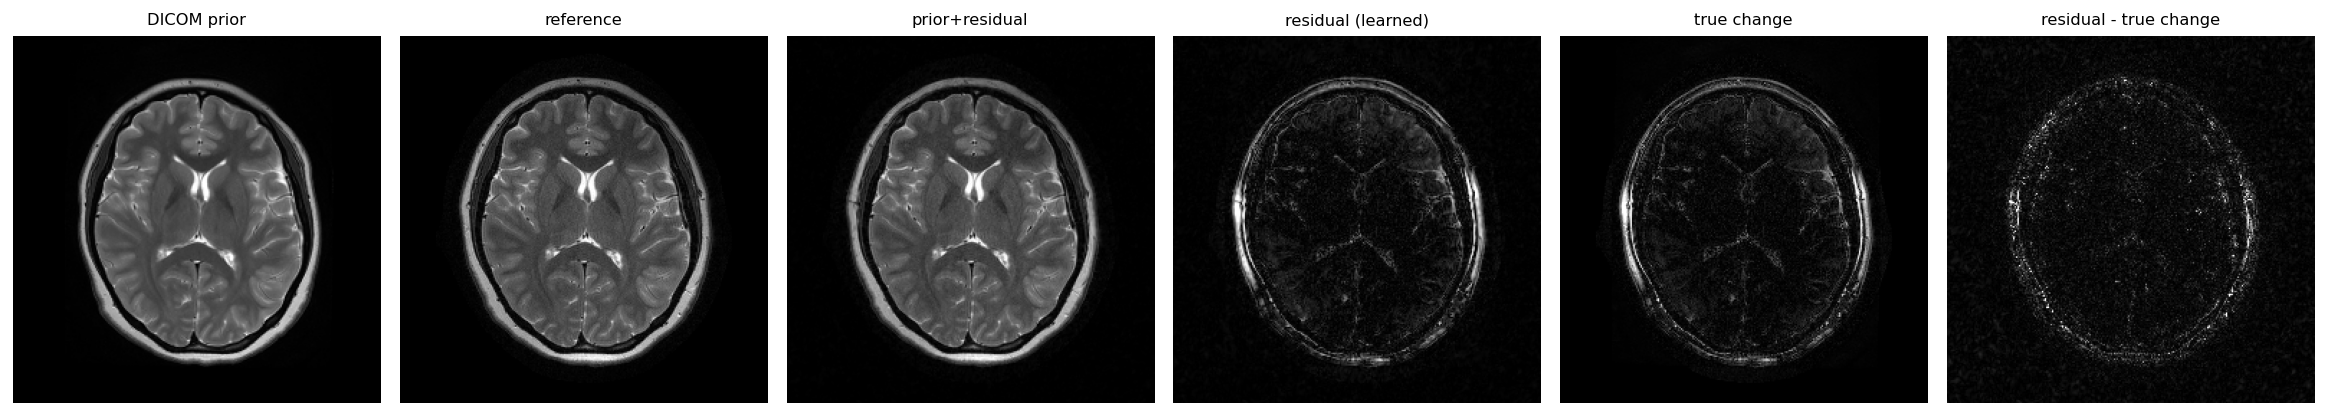
\includegraphics[width=\linewidth]{panel_p100.png}
\caption{$p=100\%$ of follow-up pixels observed. Left to right: DICOM prior, reference follow-up, our reconstruction ($f^{\mathrm{prior}}+r$), learned residual $r$, true change, and the error $|r-\text{true change}|$.}
\end{figure}
\end{document}